\documentclass[a4paper, 11pt]{article}
\usepackage[T1]{fontenc}
\usepackage[utf8]{inputenc}
\usepackage[english]{babel}
\usepackage{mathtools}
\usepackage{amsfonts}
\usepackage{amsmath}
\usepackage{amsthm}
\usepackage{mathrsfs}
\usepackage{enumitem}
\usepackage{booktabs}
\usepackage{array}
\usepackage[skip=5pt, font=footnotesize]{caption}
% Useful floor and ceiling functions
\DeclarePairedDelimiter{\floor}{\lfloor}{\rfloor}
\DeclarePairedDelimiter{\ceil}{\lceil}{\rceil}
% Argmax/Argmin notation
\DeclareMathOperator*{\argmax}{argmax} 
\DeclareMathOperator*{\argmin}{argmin}
\DeclareMathOperator*{\rep}{rep} 
% Modified margins
%\usepackage[margin=2cm]{geometry}
% This avoids hypenation
\hyphenpenalty=1000
\usepackage{tikz}
\usetikzlibrary{arrows,calc,positioning,shadows,shapes}
\usepackage{graphicx}
\usepackage{subfig}
\graphicspath{{./images/}}
\captionsetup[figure]{labelfont={bf},name={Figure},labelsep=period}
\captionsetup[table]{labelfont={bf},name={Table},labelsep=period}

\usepackage{float}
\usepackage{xfrac}
\usepackage{pgfplots}
\usepackage{titling}
\usepackage[bottom]{footmisc}
\usepackage{wrapfig}
\usepackage{lipsum}

\begin{document}

\begin{titlepage}

\vspace*{1cm}

\begin{center}
\large \textsc{Università degli Studi di Padova \\ Department of Information Engineering}

\vspace*{1cm}

\rule{\linewidth}{1pt} \Huge{ \textsc{Digital Forensics}} \\ {\textsc{First Laboratory Report}} \rule{\linewidth}{2pt}

\vspace*{1cm}

\large \textsc{Faccin Dario} \\
\normalsize \textsc{ID Number: 1177736}

\end{center}
\end{titlepage}

\section*{Introduction}
Learning can be divided into three main group, according to the strategy:
\begin{itemize}
	\item supervised learning: in this situation the classifier is trained assuming that the true label of each input variable is priory known;
	\item unsupervised learning: in this situation the classifier learns the underlying
	regularities and structure of the data without any prior information about their classes;
	\item reinforcement learning: in this situation the classifier learns the underlying
	regularities and structure of the data by actively interacting with the environment.
\end{itemize}

Each approach has its own pros and cons: the first one is a very powerful tool but requires very large dataset and manual data pre-processing in order to provide the correct labels. 

Formally, it is possible to define the \textit{learner} as an entity having access to the following data:
\begin{itemize}
	\item domain set $\mathcal{X}$: the set of all possible objects to make predictions about;
	\item label set $\mathcal{Y}$: the set of possible labels;
	\item training data $\mathcal{S}= \left( (x_1, y_1), \dots, (x_m, y_m) \right)$: a finite sequence of labeled domain points.
\end{itemize}

The output of the learner is called classifier (or predictor) and is a prediction rule $$h: \mathcal{X} \mapsto \mathcal{Y}$$

\subsection*{Classification}
Classification is the process of predicting the class of given data points. Classes are sometimes called as targets/labels. Classification predictive modeling is the task of approximating a mapping function ($f$) from input variables ($X$) to discrete output variables ($y$).

According to the previous categorization, classification is a branch of supervised learning: in fact it is necessary to provide the correct labels to the learning algorithm.

\section*{Linear models}
Many learning algorithms that are being widely used in practice rely on linear predictors, first and foremost because of the ability to learn them efficiently in many cases. In addition, linear predictors are intuitive, are easy to interpret, and fit the data reasonably well in many natural learning problems.

The class of affine functions is defined as
\begin{equation}
L_d = \left\{ h_{\mathbf{w},b}: \mathbf{w} \in \mathbb{R}^d, b \in \mathbb{R} \right\}
\end{equation}
where
\begin{equation}
h_{\mathbf{w},b} = \langle \mathbf{w}, \mathbf{x} \rangle + b = \left( \sum\limits_{i=1}^{d} w_i x_i \right) + b
\end{equation}

Typically the component $b$, called \textit{bias}, is included into $\mathbf{w}$ as an extra coordinate and the value $1$ is added as a coordinate to all $\mathbf{x} \in \mathcal{X}$: then $\mathbf{w'} = (b, w_1, \dots, w_d)$ and $\mathbf{x'} = (1, x_1, \dots, x_d)$.

\subsection*{Halfspaces and linear perceptron}
For the binary classification problem an useful hypothesis class is the class of \textit{halfspaces}. This class is defined as:
\begin{equation}
HS_d = \text{sign} \circ L_d = \left\{\mathbf{x} \mapsto \text{sign} \left( h_{\mathbf{w},b}(\mathbf{x}) \right) : h_{\mathbf{w},b} \in L_d \right\}
\end{equation}

Each halfspace is parametrized by $\mathbf{w} \in \mathbb{R}^d$ and $b \in \mathbb{R}$ and the predicted label is returned as $\text{sign} \left( \langle \mathbf{w}, \mathbf{x} \rangle + b \right)$.

\section*{Support Vector Machines}
The margin of a hyperplane with respect to a training set is defined to be the
minimal distance between a point in the training set and the hyperplane. If a
hyperplane has a large margin, then it will still separate the training set even if we slightly perturb each instance.

The name ``support vector'' derives from the fact that the optimal solution for the separation, $\mathbf{w}_0$ is a linear span of the examples which are at distance $\frac{1}{||\mathbf{w}_0||}$ from the separating hyperplane.

\subsection*{Hard SVM}
Hard SVM is a learning rule in which the learner output is an hyperplane that separates the training set with the highest possible margin.

It can be shown that the distance between a point $\mathbf{x}$ and the hyperplane defined by $(\mathbf{w}, b)$, with $||\mathbf{w}||=1$ is $|\langle \mathbf{w}, \mathbf{x} \rangle + b | $.

Given this, the hard SVM rule consists in maximizing the the closest point in the training set to the separating hyperplane. This can be expressed as
\begin{equation}
    \argmax\limits_{(\mathbf{w},b):||\mathbf{w}||=1} \min\limits_{i \in [m]} | \langle \mathbf{w}, \mathbf{x}_i \rangle + b| \quad \forall \, i : y_i \left( \langle  \mathbf{w}, \mathbf{x}_i \rangle + b \right) > 0
\end{equation}

\subsection*{Soft SVM}
When the training set is not linearly separable, the Hard-SVM method can not work. In this case there is the need to relax the assumption that a separating hyperplane exists.

In this case some elements in the training set are allowed to ``violate'' the constraint
\begin{equation}\label{eq:constraint1}
	y_i \left( \langle \mathbf{w}, \mathbf{x}_i \rangle +b \right) > 1
\end{equation}

This can be modeled by introducing non-negative slack variables, $ \xi_1$, $\dots$, $\xi_m$, representing how much the constraint is violated, and replacing the constraint \ref{eq:constraint1} with
\begin{equation}
	y_i \left( \langle \mathbf{w}, \mathbf{x}_i \rangle +b \right) > 1 - \xi_i
\end{equation}

The tradeoff between the minimization of the norm of $\mathbf{w}$ and the average constraint violations is controlled by a parameter $\lambda$.

\subsection*{The kernel method}
A kernel is a type of a similarity measure between instances. Given an embedding $\psi$ of some domain space X into some Hilbert space, it is possible to defined
the kernel function $K(\mathbf{x}, \mathbf{x'}) = \langle \psi(\mathbf{x}), \psi(\mathbf{x'})$.

The function $K$ specifies the similarity between instances and the embedding $\psi$ maps the domain set $\mathcal{X}$ into a peculiar space where this similarity is realized as inner product.

\subsubsection*{Polynomial kernel}
The $k$ degree polynomial kernel is defined as
\begin{equation}
    K(\mathbf{x}, \mathbf{x'}) = \left( c + \langle \mathbf{x}, \mathbf{x'} \rangle \right)^k
\end{equation}

\subsubsection*{Gaussian radial basis function kernel}
Let the original instance space be $\mathbb{R}$ and consider the mapping $\psi$ where for each non-negative integer $n\geq 0$ there exists an element $\psi(x)_n$ that equals $\frac{1}{\sqrt{n!}} x^n \exp \left(- \frac{x^2}{2} \right)$. Then

Here the feature space is of infinite dimension while evaluating the kernel is very simple. More generally, given a scalar $\sigma > 0$, the Gaussian kernel is defined to be
\begin{equation}
K(\mathbf{x}, \mathbf{x'}) = \exp \left( - \dfrac{||\mathbf{x}-\mathbf{x'}||^2}{2\sigma} \right)
\end{equation}

Intuitively, the Gaussian kernel sets the inner product in the feature space between $\mathbf{x}, \mathbf{x'}$ to be close to zero if the instances are far away from each other
(in the original domain) and close to 1 if they are close. $\sigma$ is a parameter that
controls the scale determining what it is meant by ``close''.

\section*{Results}
The goal of this experience is to develop a machine learning algorithm to determine whether a packet belongs to Facebook or Twitter.

This analysis is performed into two different scenarios, according to the directionality of the sniffed packets: for the first one the available data for training and testing corresponds to outgoing data packets, while for the second one the data corresponds to incoming data traffic.

Since the packet are encrypted, it is necessary to utilize some high level feature. For this experiment it has been decided to use the following measurements:
\begin{itemize}
    \item average packet length: $ L = \frac{1}{N} \sum\limits_{i} l(p_i)$
    \item packet length variance: $ \sigma_L = \sqrt{\frac{1}{N} \sum\limits_i \left( l(p_i) - L \right)^2}$
\end{itemize}

For both scenarios, the model training has been conducted using a 5-fold validation.

\subsection*{Scenario 1}
For the first scenario the linear predictor has been used: the accuracy on validation test is $99.411$, so this model is usable in this case. The prediction on test set in fact yields $100\%$ accuracy, so no other predictors have been tested.

The following Figure \ref{fig:s1_linear_vector} reports the results on the test data: it is possible to see that the number of support vectors is small ($3$), indicating that no overfitting occurs.

\begin{figure}[H]
    \centering
    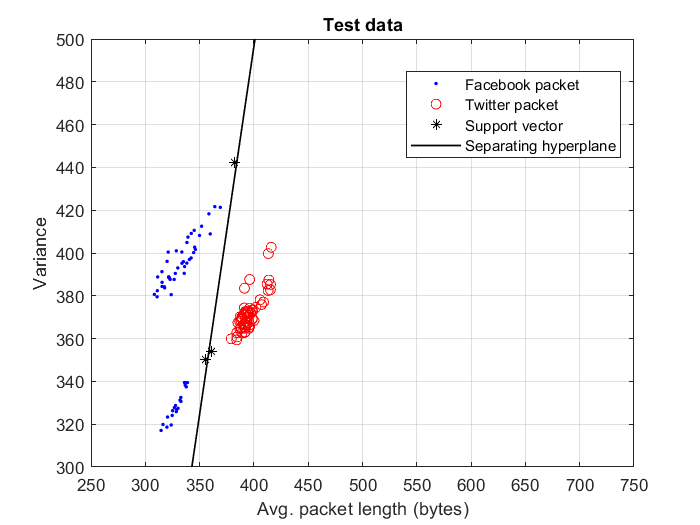
\includegraphics[width=0.4\textwidth]{s1_linear_vector}
    \caption{Result for scenario 1.}
    \label{fig:s1_linear_vector}
\end{figure}

\subsection*{Scenario 2}
For the scenario 2, the linear model has been used first; from Figure \ref{fig:s2_linear_vector} it is possible to see the behavior of this predictor. 

Both the validation and test set accuracies ($81.925$ and $88.189$, respectively) are quite high, but the main drawback is that the number of support vectors is $283$, almost half the number of the training samples.

\begin{figure}[H]
	\centering
	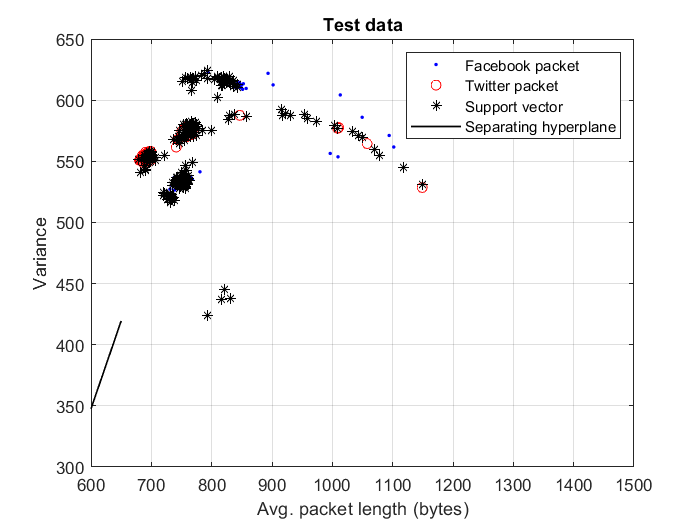
\includegraphics[width=0.4\textwidth]{s2_linear_vector}
	\caption{First result for scenario 2.}
	\label{fig:s2_linear_vector}
\end{figure}

To overcome this issue it has been decided to utilize a different training model. The RBF kernel, as seen in the previous chapter, accepts as input the parameter $\sigma$. For \texttt{libsvm} function, the input parameter is $\gamma = \frac{1}{2\sigma^2}$.

The tuning of this parameter has been conducted using a parameter sweep optimization: this consists on exhaustive searching through a manually specified subset of the hyperparameter space of the learning algorithm.

In this experiment it has been decided to use two hyperparameters:
\begin{itemize}
    \item $\gamma = \{0, \dots, 10^{-3} \}$ using an interval of $\delta_{\gamma}=10^{-4}$;
    \item $C = \{1, \dots, 5 \}$ using an interval of $\delta_{C}=0.5$
\end{itemize}
As an overall performance measure it has been decided to utilize the following quantities:
\begin{itemize}
	\item validation error;
	\item support vector ratio (SV \%): it is the ratio between the number of support vectors generated and the number of training samples used.
\end{itemize}

\begin{equation}\label{eq:min}
\argmin\limits_{\gamma} L(S_{val}) + 1.5 \cdot SV_{\%}
\end{equation}

\begin{figure}[H]
	\centering
	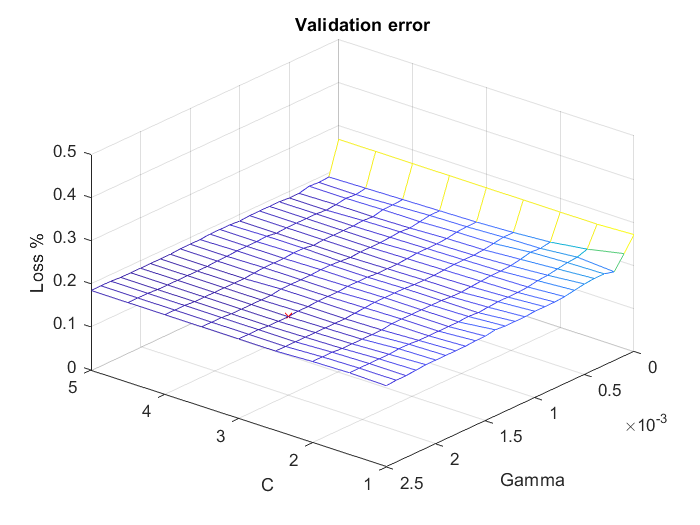
\includegraphics[width=0.4\textwidth]{s2_tradeoff_valerr_gamma_c}
	\caption{Tradeoff curve.}
	\label{fig:s2_tradeoff_valerr_gamma_c}
\end{figure}
The Figure \ref{fig:s2_tradeoff_valerr_gamma_c} shows the behavior of error on the validation dataset and the support vectors ratio for varying $\gamma$ and $C$.

The equation \ref{eq:min} reaches its minimum (0.1827) for $\gamma=0.0020$ and $C=3$. The validation accuracy is $98.035$, while the accuracy on the test set is $98.425$.

The main difference with respect to the linear model is that now the number of support vectors is $56$, which is $20\%$ that before.

\begin{thebibliography}{1}
	\bibitem{uml}
	{Shalev-Shwartz S., Ben-David, S.}, ``Understanding Machine Learning: From Theory to Algorithms'', \textit{Cambridge University Press}, 2014.
	\bibitem{milani}
	{Milani S.}, ``Digital Forensics: course lectures'', 2018.
\end{thebibliography}
\end{document}